\begin{figure}[!htb]
	\centering
	\begin{subfigure}{0.45\textwidth}
		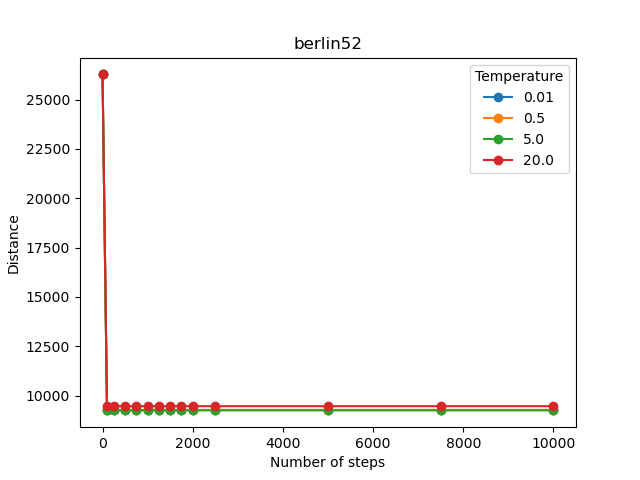
\includegraphics[width=\textwidth]{img/berlin52_temperature}
		\subcaption{berlin52.}
	\end{subfigure}
	\begin{subfigure}{0.45\textwidth}
		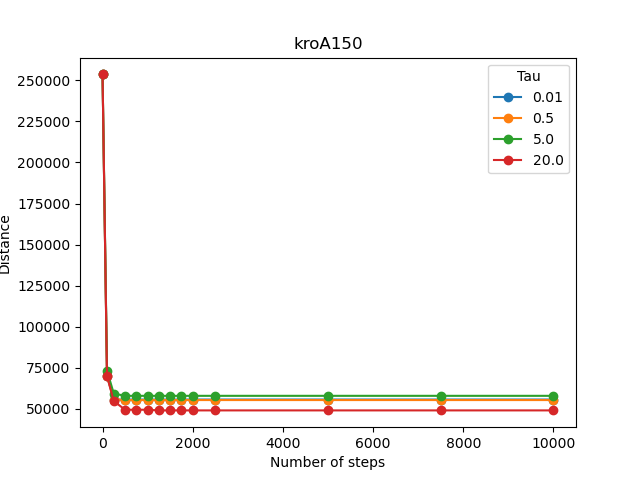
\includegraphics[width=\textwidth]{img/kroA150_temperature}
		\subcaption{kroA150.}
	\end{subfigure}
	\caption{Distances over number of steps for 2 datasets with temperature parameter.}
	\label{fig:temperature_1}
\end{figure}

\begin{figure}[!htb]
	\centering
	\begin{subfigure}{0.45\textwidth}
		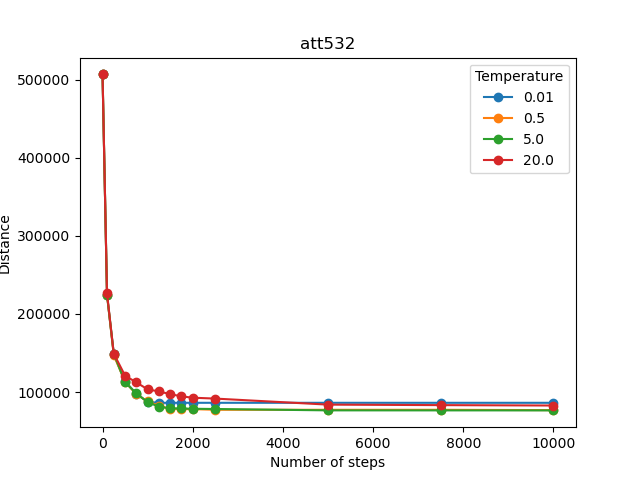
\includegraphics[width=\textwidth]{img/att532_temperature}
		\subcaption{att532.}
	\end{subfigure}
	\begin{subfigure}{0.45\textwidth}
		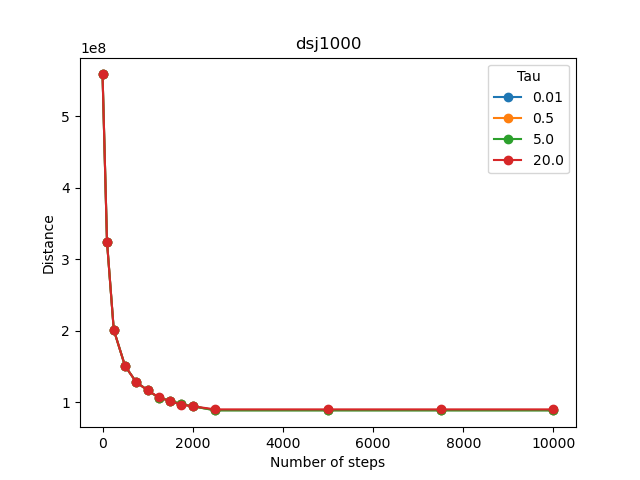
\includegraphics[width=\textwidth]{img/dsj1000_temperature}
		\subcaption{dsj1000.}
	\end{subfigure}
	\caption{Distances over number of steps for 2 datasets with temperature parameter.}
	\label{fig:temperature_2}
\end{figure}